\documentclass{standalone}
\usepackage{tikz}
\usetikzlibrary{patterns, positioning}


\begin{document}
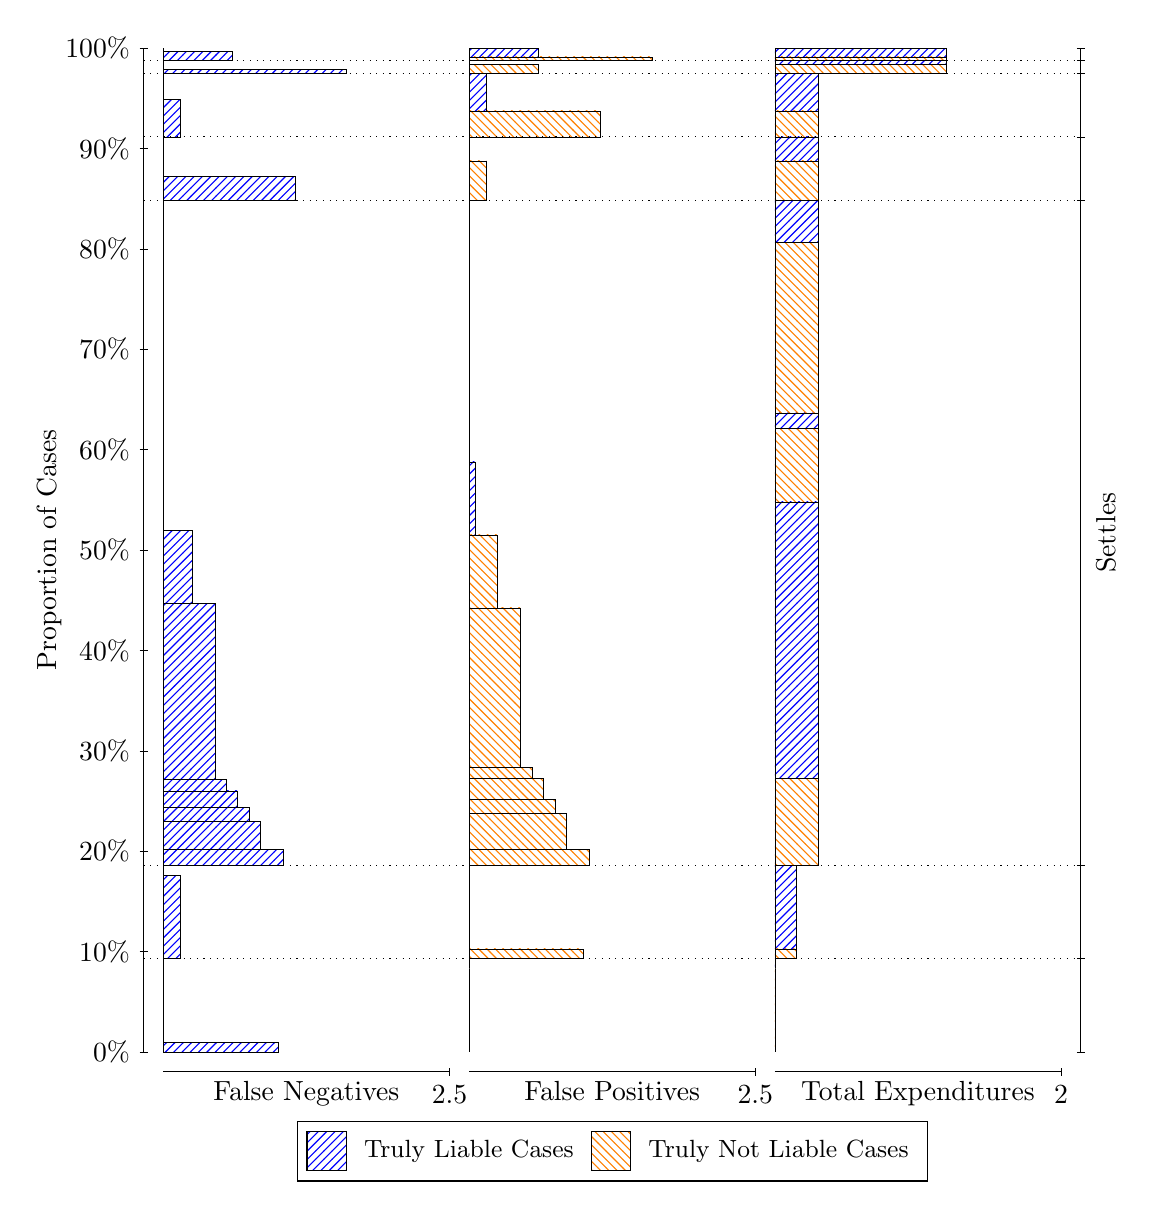
\begin{tikzpicture}
\draw[black, very thin] (1.5,1.75) -- (1.5,14.5);
\node[rotate=90, text=black, anchor=center] at (0.3, 8.125) {Proportion of Cases};
\draw[black, very thin] (1.45,1.75) -- (1.55,1.75);
\node[text=black, anchor=east] at (1.45, 1.75) {0\%};
\draw[black, very thin] (1.45,3.025) -- (1.55,3.025);
\node[text=black, anchor=east] at (1.45, 3.025) {10\%};
\draw[black, very thin] (1.45,4.3) -- (1.55,4.3);
\node[text=black, anchor=east] at (1.45, 4.3) {20\%};
\draw[black, very thin] (1.45,5.575) -- (1.55,5.575);
\node[text=black, anchor=east] at (1.45, 5.575) {30\%};
\draw[black, very thin] (1.45,6.85) -- (1.55,6.85);
\node[text=black, anchor=east] at (1.45, 6.85) {40\%};
\draw[black, very thin] (1.45,8.125) -- (1.55,8.125);
\node[text=black, anchor=east] at (1.45, 8.125) {50\%};
\draw[black, very thin] (1.45,9.4) -- (1.55,9.4);
\node[text=black, anchor=east] at (1.45, 9.4) {60\%};
\draw[black, very thin] (1.45,10.675) -- (1.55,10.675);
\node[text=black, anchor=east] at (1.45, 10.675) {70\%};
\draw[black, very thin] (1.45,11.95) -- (1.55,11.95);
\node[text=black, anchor=east] at (1.45, 11.95) {80\%};
\draw[black, very thin] (1.45,13.225) -- (1.55,13.225);
\node[text=black, anchor=east] at (1.45, 13.225) {90\%};
\draw[black, very thin] (1.45,14.5) -- (1.55,14.5);
\node[text=black, anchor=east] at (1.45, 14.5) {100\%};

\draw[black, very thin] (13.4,1.75) -- (13.4,14.5);
\draw[black, very thin] (13.35,1.75) -- (13.45,1.75);
\node[anchor=west] at (13.35, 1.75) {};
\draw[black, very thin] (13.35,2.9362) -- (13.45,2.9362);
\node[anchor=west] at (13.35, 2.9362) {};
\draw[black, very thin] (13.35,4.1195) -- (13.45,4.1195);
\node[anchor=west] at (13.35, 4.1195) {};
\draw[black, very thin] (13.35,12.569) -- (13.45,12.569);
\node[anchor=west] at (13.35, 12.569) {};
\draw[black, very thin] (13.35,13.371) -- (13.45,13.371);
\node[anchor=west] at (13.35, 13.371) {};
\draw[black, very thin] (13.35,14.178) -- (13.45,14.178);
\node[anchor=west] at (13.35, 14.178) {};
\draw[black, very thin] (13.35,14.341) -- (13.45,14.341);
\node[anchor=west] at (13.35, 14.341) {};
\draw[black, very thin] (13.35,14.5) -- (13.45,14.5);
\node[anchor=west] at (13.35, 14.5) {};

\draw[black, very thin, pattern color=blue, pattern=north east lines] (1.75,1.75) rectangle (3.2033,1.8748);
\draw[black, very thin, pattern color=orange, pattern=north west lines] (1.75,1.8748) rectangle (1.75,2.9362);
\draw[black, very thin, pattern color=blue, pattern=north east lines] (1.75,2.9362) rectangle (1.968,3.9961);
\draw[black, very thin, pattern color=orange, pattern=north west lines] (1.75,3.9961) rectangle (1.75,4.1195);
\draw[black, very thin, pattern color=blue, pattern=north east lines] (1.75,4.1195) rectangle (3.276,4.3214);
\draw[black, very thin, pattern color=blue, pattern=north east lines] (1.75,4.3214) rectangle (2.9853,4.6802);
\draw[black, very thin, pattern color=blue, pattern=north east lines] (1.75,4.6802) rectangle (2.84,4.8552);
\draw[black, very thin, pattern color=blue, pattern=north east lines] (1.75,4.8552) rectangle (2.6947,5.0661);
\draw[black, very thin, pattern color=blue, pattern=north east lines] (1.75,5.0661) rectangle (2.5493,5.2133);
\draw[black, very thin, pattern color=blue, pattern=north east lines] (1.75,5.2133) rectangle (2.404,7.4442);
\draw[black, very thin, pattern color=blue, pattern=north east lines] (1.75,7.4442) rectangle (2.1133,8.3717);
\draw[black, very thin, pattern color=orange, pattern=north west lines] (1.75,8.3717) rectangle (1.75,12.569);
\draw[black, very thin, pattern color=blue, pattern=north east lines] (1.75,12.569) rectangle (3.4213,12.874);
\draw[black, very thin, pattern color=orange, pattern=north west lines] (1.75,12.874) rectangle (1.75,13.371);
\draw[black, very thin, pattern color=blue, pattern=north east lines] (1.75,13.371) rectangle (1.968,13.846);
\draw[black, very thin, pattern color=orange, pattern=north west lines] (1.75,13.846) rectangle (1.75,14.178);
\draw[black, very thin, pattern color=blue, pattern=north east lines] (1.75,14.178) rectangle (4.0753,14.225);
\draw[black, very thin, pattern color=orange, pattern=north west lines] (1.75,14.225) rectangle (1.75,14.341);
\draw[black, very thin, pattern color=blue, pattern=north east lines] (1.75,14.341) rectangle (2.622,14.453);
\draw[black, very thin, pattern color=orange, pattern=north west lines] (1.75,14.453) rectangle (1.75,14.5);
\draw[black, very thin, pattern color=orange, pattern=north west lines] (5.6333,1.75) rectangle (5.6333,2.8114);
\draw[black, very thin, pattern color=blue, pattern=north east lines] (5.6333,2.8114) rectangle (5.6333,2.9362);
\draw[black, very thin, pattern color=orange, pattern=north west lines] (5.6333,2.9362) rectangle (7.0867,3.0596);
\draw[black, very thin, pattern color=blue, pattern=north east lines] (5.6333,3.0596) rectangle (5.6333,4.1195);
\draw[black, very thin, pattern color=orange, pattern=north west lines] (5.6333,4.1195) rectangle (7.1593,4.3213);
\draw[black, very thin, pattern color=orange, pattern=north west lines] (5.6333,4.3213) rectangle (6.8687,4.7802);
\draw[black, very thin, pattern color=orange, pattern=north west lines] (5.6333,4.7802) rectangle (6.7233,4.9552);
\draw[black, very thin, pattern color=orange, pattern=north west lines] (5.6333,4.9552) rectangle (6.578,5.2206);
\draw[black, very thin, pattern color=orange, pattern=north west lines] (5.6333,5.2206) rectangle (6.4327,5.3678);
\draw[black, very thin, pattern color=orange, pattern=north west lines] (5.6333,5.3678) rectangle (6.2873,7.3897);
\draw[black, very thin, pattern color=orange, pattern=north west lines] (5.6333,7.3897) rectangle (5.9967,8.3173);
\draw[black, very thin, pattern color=blue, pattern=north east lines] (5.6333,8.3173) rectangle (5.706,9.2447);
\draw[black, very thin, pattern color=blue, pattern=north east lines] (5.6333,9.2447) rectangle (5.6333,12.569);
\draw[black, very thin, pattern color=orange, pattern=north west lines] (5.6333,12.569) rectangle (5.8513,13.066);
\draw[black, very thin, pattern color=blue, pattern=north east lines] (5.6333,13.066) rectangle (5.6333,13.371);
\draw[black, very thin, pattern color=orange, pattern=north west lines] (5.6333,13.371) rectangle (7.3047,13.703);
\draw[black, very thin, pattern color=blue, pattern=north east lines] (5.6333,13.703) rectangle (5.8513,14.178);
\draw[black, very thin, pattern color=orange, pattern=north west lines] (5.6333,14.178) rectangle (6.5053,14.294);
\draw[black, very thin, pattern color=blue, pattern=north east lines] (5.6333,14.294) rectangle (5.6333,14.341);
\draw[black, very thin, pattern color=orange, pattern=north west lines] (5.6333,14.341) rectangle (7.9587,14.388);
\draw[black, very thin, pattern color=blue, pattern=north east lines] (5.6333,14.388) rectangle (6.5053,14.5);
\draw[black, very thin, pattern color=orange, pattern=north west lines] (9.5167,1.75) rectangle (9.5167,2.8114);
\draw[black, very thin, pattern color=blue, pattern=north east lines] (9.5167,2.8114) rectangle (9.5167,2.9362);
\draw[black, very thin, pattern color=orange, pattern=north west lines] (9.5167,2.9362) rectangle (9.7892,3.0596);
\draw[black, very thin, pattern color=blue, pattern=north east lines] (9.5167,3.0596) rectangle (9.7892,4.1195);
\draw[black, very thin, pattern color=orange, pattern=north west lines] (9.5167,4.1195) rectangle (10.062,5.2206);
\draw[black, very thin, pattern color=blue, pattern=north east lines] (9.5167,5.2206) rectangle (10.062,8.7371);
\draw[black, very thin, pattern color=orange, pattern=north west lines] (9.5167,8.7371) rectangle (10.062,9.6646);
\draw[black, very thin, pattern color=blue, pattern=north east lines] (9.5167,9.6646) rectangle (10.062,9.8665);
\draw[black, very thin, pattern color=orange, pattern=north west lines] (9.5167,9.8665) rectangle (10.062,12.036);
\draw[black, very thin, pattern color=blue, pattern=north east lines] (9.5167,12.036) rectangle (10.062,12.569);
\draw[black, very thin, pattern color=orange, pattern=north west lines] (9.5167,12.569) rectangle (10.062,13.066);
\draw[black, very thin, pattern color=blue, pattern=north east lines] (9.5167,13.066) rectangle (10.062,13.371);
\draw[black, very thin, pattern color=orange, pattern=north west lines] (9.5167,13.371) rectangle (10.062,13.703);
\draw[black, very thin, pattern color=blue, pattern=north east lines] (9.5167,13.703) rectangle (10.062,14.178);
\draw[black, very thin, pattern color=orange, pattern=north west lines] (9.5167,14.178) rectangle (11.697,14.294);
\draw[black, very thin, pattern color=blue, pattern=north east lines] (9.5167,14.294) rectangle (11.697,14.341);
\draw[black, very thin, pattern color=orange, pattern=north west lines] (9.5167,14.341) rectangle (11.697,14.388);
\draw[black, very thin, pattern color=blue, pattern=north east lines] (9.5167,14.388) rectangle (11.697,14.5);
\draw[black, dotted] (1.5,2.9362) -- (13.4,2.9362);
\draw[black, dotted] (1.5,4.1195) -- (13.4,4.1195);
\draw[black, dotted] (1.5,12.569) -- (13.4,12.569);
\draw[black, dotted] (1.5,13.371) -- (13.4,13.371);
\draw[black, dotted] (1.5,14.178) -- (13.4,14.178);
\draw[black, dotted] (1.5,14.341) -- (13.4,14.341);
\draw[black, very thin] (1.75,1.5) -- (5.3833,1.5);
\node[text=black, anchor=north] at (3.5667, 1.5) {False Negatives};
\draw[black, very thin] (5.3833,1.45) -- (5.3833,1.55);
\node[text=black, anchor=north] at (5.3833, 1.45) {2.5};

\draw[black, very thin] (5.6333,1.5) -- (9.2667,1.5);
\node[text=black, anchor=north] at (7.45, 1.5) {False Positives};
\draw[black, very thin] (9.2667,1.45) -- (9.2667,1.55);
\node[text=black, anchor=north] at (9.2667, 1.45) {2.5};

\draw[black, very thin] (9.5167,1.5) -- (13.15,1.5);
\node[text=black, anchor=north] at (11.333, 1.5) {Total Expenditures};
\draw[black, very thin] (13.15,1.45) -- (13.15,1.55);
\node[text=black, anchor=north] at (13.15, 1.45) {2};



\node[text=black, centered, rotate=90] at (13.72, 8.3445) {Settles};





\draw (7.449999999999999,1.5) node[draw=none] (baseCoordinate) {};
\begin{scope}[align=center]
        \matrix[scale=0.5, draw=black, below=0.5cm of baseCoordinate, nodes={draw}, column sep=0.1cm]{
            \node[rectangle, draw, minimum width=0.5cm, minimum height=0.5cm, pattern color=blue, pattern=north east lines] {}; &
            \node[draw=none, font=\small, text=black] (B) {Truly Liable Cases}; &
            \node[rectangle, draw, minimum width=0.5cm, minimum height=0.5cm, pattern color=orange, pattern=north west lines] {}; &
            \node[draw=none, font=\small, text=black] (B) {Truly Not Liable Cases}; \\
            };
\end{scope}

\end{tikzpicture}
\end{document}